\chapter{Esercizi Teoria Esame}
\subsection{Esercizi - schema concettuale}
\subsection*{Esercizio 7}
\textbf{Richiesta. }Descrivere lo schema concettuale della seguente
realtà:
Degli impiegati interessa il codice fiscale, il nome, il
cognome, i dipartimenti ai quali afferiscono (con la
data di afferenza), ed i progetti ai quali partecipano.
Dei progetti interessa il nome, il budget, e la città in
cui hanno luogo le corrispondenti attività. Alcuni
progetti sono parti di altri progetti, e sono detti loro
sottoprogetti. Dei dipartimenti interessa il nome, il
numero di telefono, gli impiegati che li dirigono, e la
città dove è localizzata la sede. Delle città interessa
il nome e la regione.\medskip\\
\textbf{Soluzione. }
\begin{figure}[H]
    \centering  
    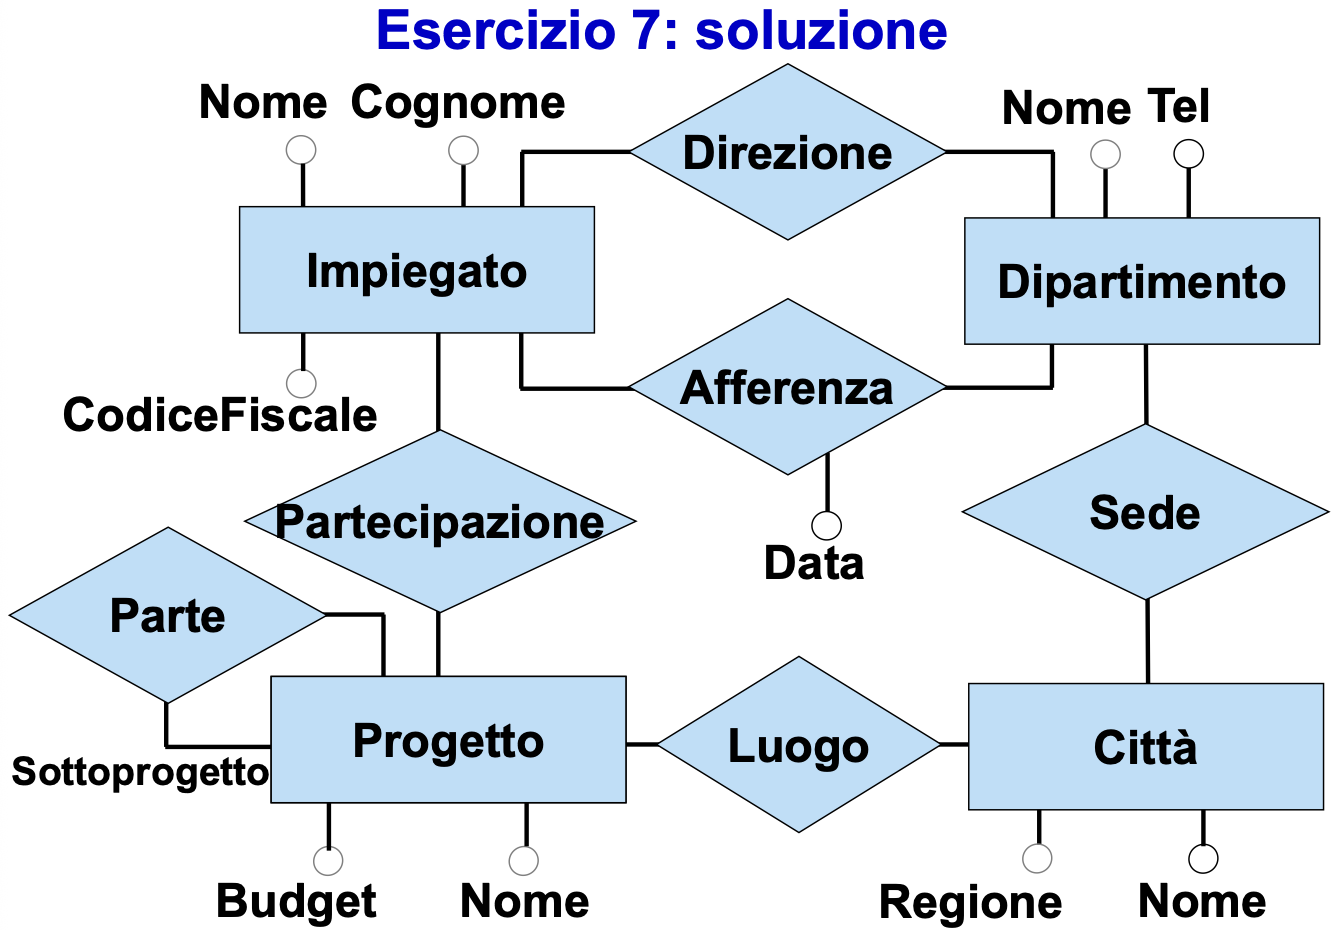
\includegraphics[width=0.6\linewidth]{../images/esercizio7.png}
    %\caption{caption}
    %\label{label}
\end{figure}
\noindent
\begin{itemize}
    \item La data è un attributo di Afferenza, perché riguarda il legame tra un impiegato e un dipartimento. Lo stesso impiegato può afferire a dipartimenti diversi in date diverse.
    \item Direzione e Afferenza sono relazioni distinte: lavorare in un dipartimento e dirigerlo sono due informazioni diverse. Il testo non impone esplicitamente che chi dirige un dipartimento debba anche afferirvi.
    \item Città è un’entità, con attributi Nome e Regione. È collegata ai dipartimenti tramite Sede e ai progetti tramite Luogo: la stessa città può ospitare sedi e attività di più progetti.
    \item Parte è una relazione ricorsiva: collega due istanze dell’entità Progetto. Una ha il ruolo di progetto principale, l’altra di Sottoprogetto. Non serve un’entità separata per i sottoprogetti.
\end{itemize}
\noindent
Nello schema mancano però le cardinalità e l’indicazione degli identificatori
\subsection*{Esercizio 12}
\textbf{Richiesta. }Descrivere lo schema concettuale corrispondente ad
un'applicazione riguardante voli aerei, per la quale valgono le
seguenti specifiche.
Dei voli interessa: codice, durata in minuti, compagnia aerea,
aeroporto di partenza e aeroporto di arrivo. Degli aeroporti
interessa: codice, nome, città (con nome e numero di abitanti) e
nazione. Delle compagnie aeree interessa il nome, l’anno di
fondazione, e la città in cui ha sede la direzione. I voli charter
sono particolari voli, che possono prevedere tappe intermedie
in aeroporti. Delle tappe intermedie di un volo charter interessa
l'ordine con cui esse si susseguono (ad esempio, il volo 124,
che parte da “Milano Linate” e arriva a “Palermo Punta Raisi”,
prevede prima l'aeroporto di Bologna e poi quello di Napoli
come tappe intermedie). Infine, dei voli charter interessa anche
il tipo di aereomobile utilizzato per il volo.\medskip\\
\textbf{Soluzione. }
\begin{figure}[H]
    \centering  
    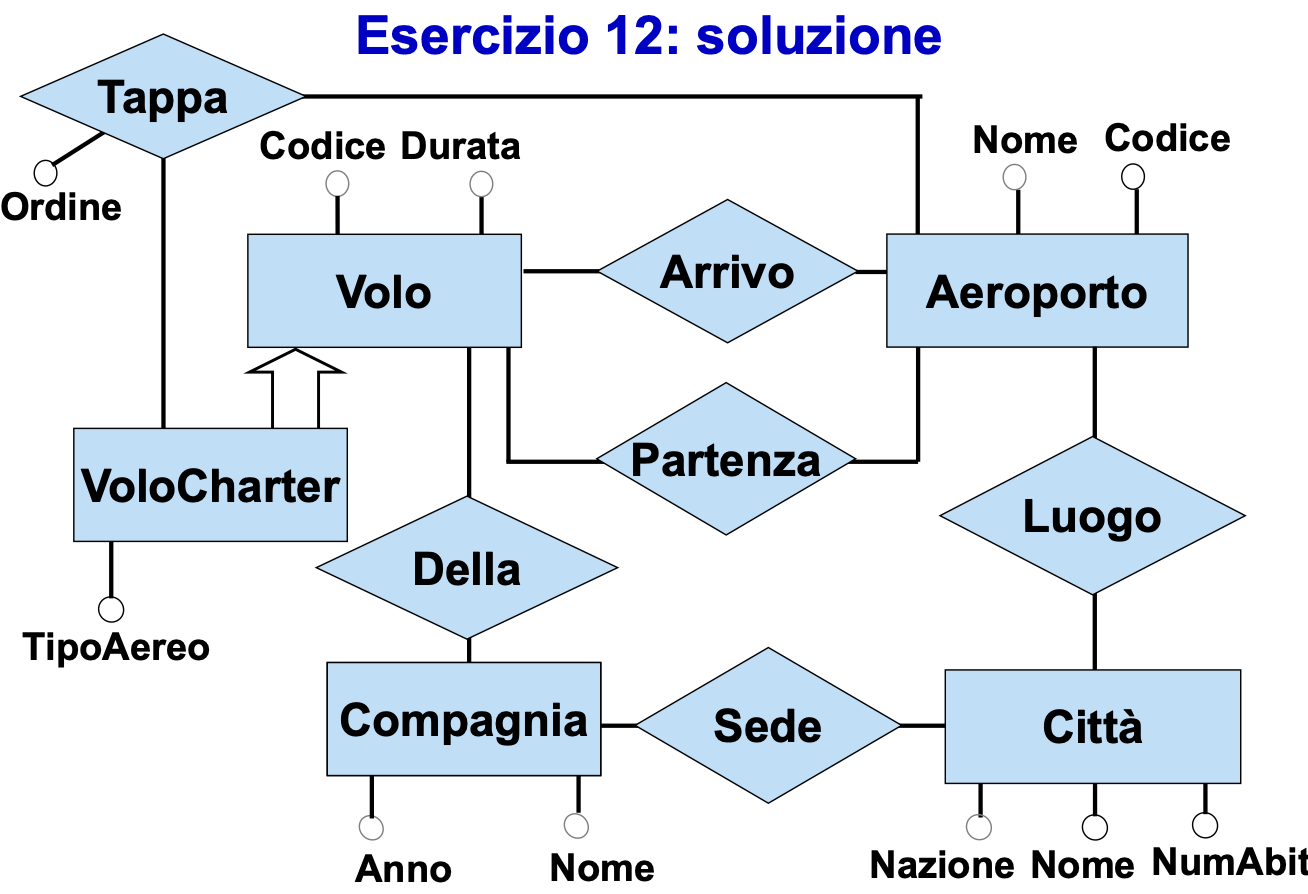
\includegraphics[width=0.6\linewidth]{../images/esercizio12.png}
    %\caption{caption}
    %\label{label}
\end{figure}
\begin{itemize}
    \item VoloCharter è un sottoinsieme di Volo
    La freccia indica una relazione “è un”: ogni volo charter è anche un volo. Quindi eredita codice, durata e le relazioni con compagnia, aeroporto di partenza e aeroporto di arrivo. In più possiede l’attributo TipoAereo e può avere tappe intermedie.
    La specializzazione è parziale: non tutti i voli sono charter.
    \item Ordine è un attributo della relazione Tappa. Non appartiene all’aeroporto: Bologna può essere la prima tappa di un volo e la terza di un altro
    \item Città è condivisa da aeroporti e compagnie
    Luogo indica dove si trova un aeroporto; Sede indica dove ha sede la direzione di una compagnia. La Nazione è stata collocata in Città: la nazione dell’aeroporto si ricava dalla città in cui si trova.

\end{itemize}
\noindent
Una precisazione sul modello: la relazione Tappa presuppone che uno stesso aeroporto compaia al massimo una volta fra le tappe di uno stesso volo. Se si volessero ammettere passaggi ripetuti, servirebbe un’entità Tappa, identificata dal volo e dall’ordine, collegata all’aeroporto.\medskip\\
\textbf{Altra soluzione. }\\
\begin{figure}[H]
    \centering  
    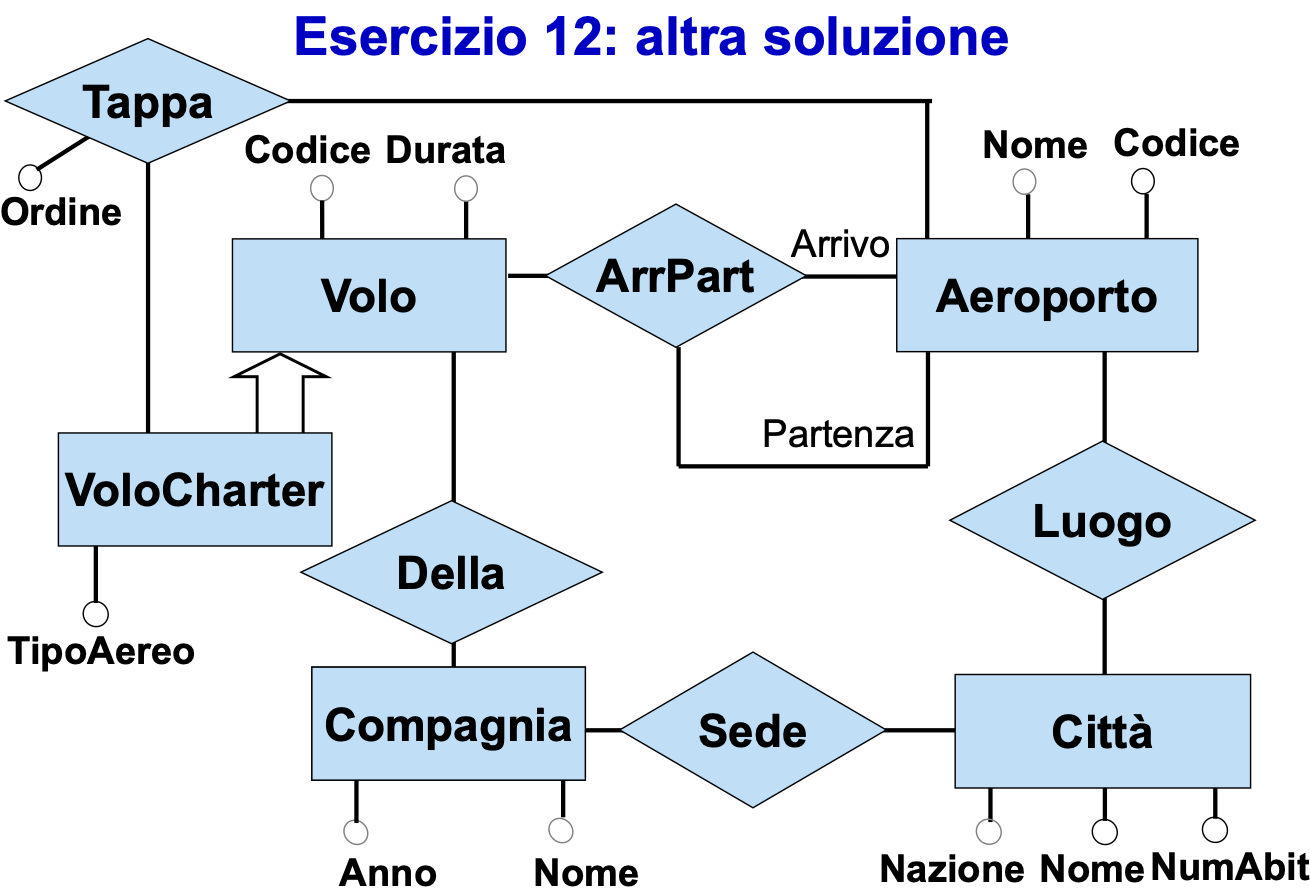
\includegraphics[width=0.6\linewidth]{../images/esercizio12b.png}
    %\caption{caption}
    %\label{label}
\end{figure}

\subsection*{Esercizio 14}
\textbf{Richiesta. }Descrivere lo schema concettuale corrispondente
alle seguenti specifiche.
Le persone hanno un codice fiscale ed una età.
Gli uomini anche la posizione militare, e le donne
anche il numero di maternità. Gli impiegati hanno
lo stipendio e possono essere o segretari, o
direttori o progettisti. Alcuni progettisti sono
responsabili di progetto. Gli studenti (che non
possono essere impiegati) hanno un numero di
matricola. Esistono persone che non sono né
impiegati né studenti.\medskip\\
\textbf{Soluzione. }
\begin{figure}[H]
    \centering  
    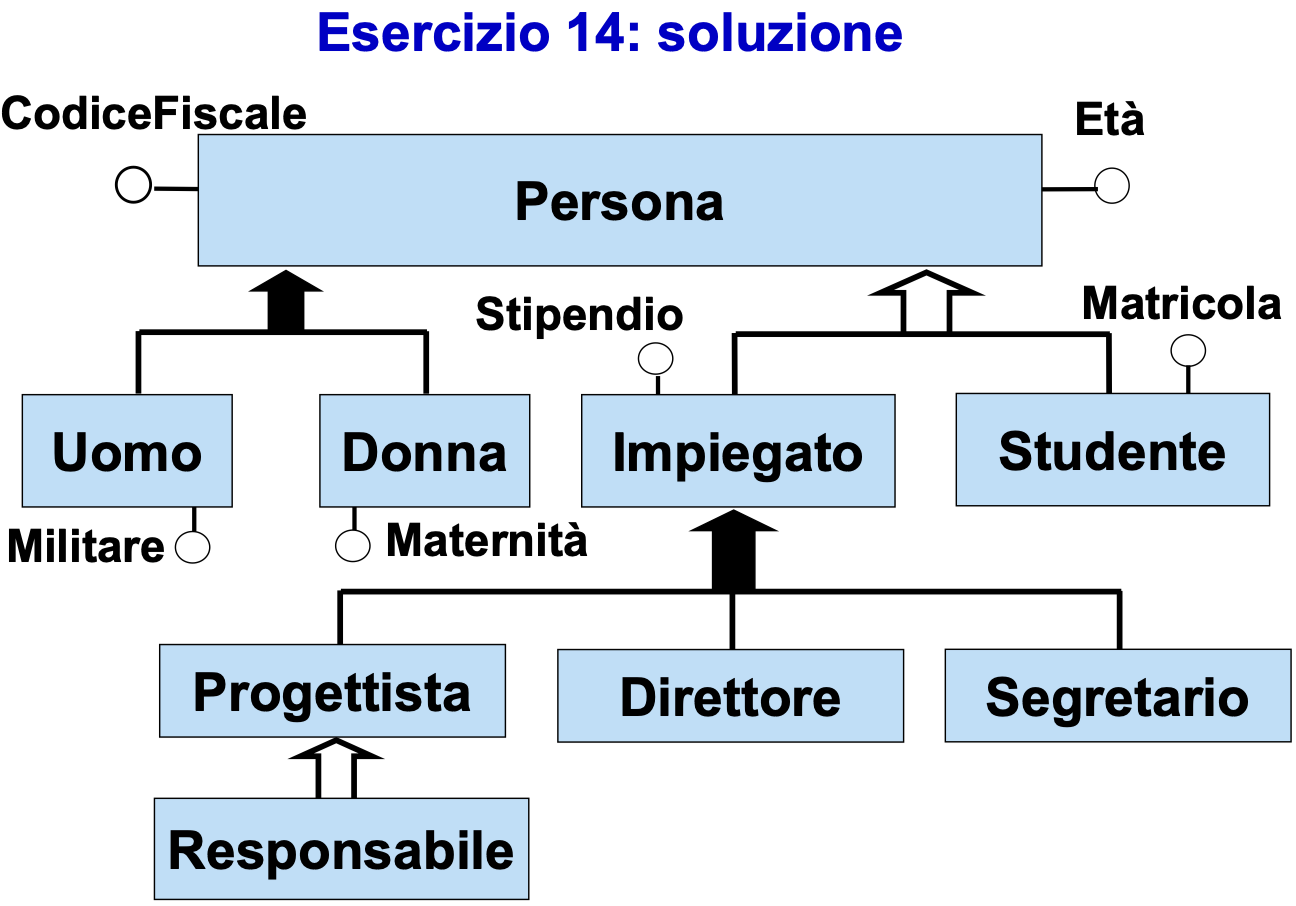
\includegraphics[width=0.6\linewidth]{../images/esercizio14.png}
    %\caption{caption}
    %\label{label}
\end{figure}
\noindent
Le due generalizzazioni di Persona sono indipendenti. Una persona può essere, per esempio, contemporaneamente Donna e Studente oppure Uomo e Impiegato. L’esclusività vale tra i figli della stessa generalizzazione, non tra tutti i sottotipi presenti nello schema.
Gli attributi si ereditano lungo la gerarchia. Un Responsabile è anche Progettista, quindi Impiegato e quindi Persona: possiede CodiceFiscale, Età e Stipendio, anche se non vengono ripetuti nel suo rettangolo.
Infine, Responsabile può essere un sottotipo anche senza attributi propri: serve a distinguere il sottoinsieme dei progettisti che hanno quella qualifica.


\section{Teoria}
\subsection{Vincoli di integrità}
\textbf{Richiesta. }Cos'è un vincolo di integrità?\\
\textbf{Soluzione. }Un vincolo di integrità è una condizione che si esprime a livello di schema intenzionale e deve essere rispettata da ogni istanza dello schema a livello estensionale.\medskip\\
\textbf{Richiesta. }Classifica i vincoli di integrità?\\
\textbf{Soluzione. }Vincoli di cardinalità sulle relazioni; sugli attributi; vincoli di identificazione di entità e di relazioni; altri vincoli.\medskip\\
\textbf{Richiesta. }Cos'è un vincolo di cardinalità?\\
\textbf{Soluzione. }Un vincolo di cardinalità si associa ad un ruolo $U$ corrispondente ad un entitò $E$ e in una relazione $R$, ed impone un limite minimo ed un limite massimo di istanze della relazione a cui può partecipare ogni dell'entità $E$ nel ruolo $U$.
